\documentclass[11pt,a4paper]{article}

% --- PACOTES BÁSICOS ---
\usepackage[utf8]{inputenc}
\usepackage[brazil]{babel}
\usepackage[T1]{fontenc}
\usepackage{graphicx}
\usepackage{url}
\usepackage{hyperref}
\usepackage{float}
\usepackage{caption}

% --- ESTILO E CORES (AZUL IFSC) ---
\usepackage[left=2.5cm, right=2.5cm, top=2.5cm, bottom=2.5cm]{geometry}
\usepackage[most]{tcolorbox}
\usepackage[table,x11names]{xcolor}
\usepackage{colortbl}
\usepackage{longtable}
\usepackage{array}
\usepackage{multirow}
\usepackage{ragged2e}
\usepackage{minted}
\usepackage{amsmath, amssymb}
\usepackage{tikz}
\usetikzlibrary{arrows.meta, shapes.geometric, shapes.symbols, positioning, fit, shapes}
\usepackage[style=abnt, backend=biber]{biblatex}
\addbibresource{references.bib}

% Definição da cor institucional
\definecolor{azulIFSC}{RGB}{30, 60, 90} 

% --- CONFIGURAÇÃO DE MINTED (CÓDIGO) ---
\usemintedstyle{colorful}
\setminted{
    fontsize=\small,
    breaklines=true,
    frame=single,
    rulecolor=azulIFSC,
    bgcolor=gray!5
}

% --- AMBIENTES CUSTOMIZADOS ---

% Box para Tutoriais
\newtcolorbox{boxTutorial}[1]{
    colback=white,
    colframe=azulIFSC,
    fonttitle=\bfseries\large,
    title={#1},
    enhanced,
    attach boxed title to top left={yshift=-2mm, xshift=2mm},
    boxed title style={colback=azulIFSC},
    breakable,
    sharp corners=northeast,
    boxrule=0.8pt,
    top=10pt
}

% Box para Avisos/Atividades
\newtcolorbox{boxAvisos}[1]{
    colback=azulIFSC!5,
    colframe=azulIFSC!80,
    fonttitle=\bfseries,
    title=#1,
    breakable,
    left=5pt, right=5pt
}

% Reajuste de parágrafo e espaçamento
\setlength{\parindent}{0pt}
\setlength{\parskip}{8pt}

\title{\textbf{\color{azulIFSC}Luisa's Project Documentation: \\ COTB Python Game Notes}}
\author{Luisa Narvaz Blankenburg \\ \small Orientação: Prof. Andre Luiz de Moraes}
\date{2025/2026}


% ==== README ====

    %=== FOR CHECK / CHECKED BOXES
    % Esse código vai gerar uma tabela grande com as tarefas organizadas por etapa, com caixas desmarcadas ($\Box$). Para marcar alguma como feita, basta trocar \Box por \boxtimes.

\begin{document}

\maketitle

% Criando o sumário
\tableofcontents


\begin{boxAvisos}{Próximas Atividades}
    \begin{itemize}
        \item \textbf{Tutorial 9:} Implementação de Score, Estímulo-Resposta e Feedback (Seção \ref{sec: Tutorial 9: Fase 1}).
            \begin{itemize}
                \item Registrar vídeo da etapa para comparação futura.
            \end{itemize}
        \item \textbf{Tutorial 10:} Interação com botões e GPIO (Seção \ref{sec:Tutorial10_Botoes}).
        \item \textbf{Escrita Científica:} Redigir capítulos de Background e Related Works.
    \end{itemize}
\end{boxAvisos}
 \section{Checklist de Atividades}

\rowcolors{2}{white}{azulIFSC!5}
\begin{longtable}{|>{\RaggedRight}m{4.2cm}|>{\RaggedRight}m{4.3cm}|m{2.5cm}|c|m{1.8cm}|}
\hline
\rowcolor{azulIFSC}
\textbf{\color{white}Etapa} & \textbf{\color{white}Tarefa} & \textbf{\color{white}Observação} & \textbf{\color{white}Status} & \textbf{\color{white}Previsão} \\
\hline
\multirow{3}{=}{Etapa 0: Fundamentação e Preparação} 
 & Criar referencial teórico. & ~ & $\boxtimes$ & Ago-3 \\
 & Estruturar repositório. & ~ & $\boxtimes$ & Ago-3 \\
 & Planejamento inicial. & ~ & $\boxtimes$ & Ago-4 \\
\hline
\multirow{8}{=}{Etapa 1: Definição e Ambiente} 
 & Refinar ideia central. & ~ & $\boxtimes$ & Ago-4 \\
 & Público-alvo (7-10 anos). & ~ & $\boxtimes$ & Ago-4 \\
 & Tipo de tarefa. & Altura/Melodia & $\boxtimes$ & Ago-4 \\
 & Verificar acesso ao público-alvo. & ~ & $\Box$ & Set-1 \\
 & Plataforma Web/Desktop. & ~ & $\boxtimes$ & Set-1 \\
 & Configurar UTM/VM. & ~ & $\boxtimes$ & Set-1 \\
 & Interações gráficas. & ~ & $\boxtimes$ & Set-2 \\
 & Uso do terminal e script Python. & ~ & $\boxtimes$ & Set-3 \\
\hline
\multirow{6}{=}{Etapa 2: Design e Feedback} 
 & Lógica e regras do jogo. & ~ & $\boxtimes$ & Set-3 \\
 & Protótipo visual. & ~ & $\boxtimes$ & Set-3 \\
 & Estímulos musicais. & ~ & $\Box$ & Set-4 \\
 & Mapear sons a eventos. & ~ & $\Box$ & Set-4 \\
 & Fluxograma de interação. & ~ & $\boxtimes$ & Set-4 \\
 & Protótipo final de interface. & ~ & $\boxtimes$ & Set-4 \\
\hline
\multirow{5}{=}{Etapa 3A: Programação no Raspberry} 
 & Instalar ambiente Raspbian. & UTM/VirtualBox. & $\boxtimes$ & Ago-4 \\
 & Implementar script de som (\texttt{pygame}). & ~ & $\boxtimes$ & Out-1 \\
 & Reprodução de áudio. & ~ & $\boxtimes$ & Out-1 \\
 & Testar teclado $\to$ som. & ~ & $\boxtimes$ & Out-2 \\
 & Protótipo funcional integrado. & ~ & $\boxtimes$ & Out-2 \\
\hline
\multirow{4}{=}{Etapa 3B: Implementação Lógica} 
 & Tela inicial (Nome/Escola). & ~ & $\boxtimes$ & Out-3 \\
 & Progressão de fases. & ~ & $\Box$ & Out-4 \\
 & Feedback sonoro integrado. & ~ & $\Box$ & Out-4 \\
\hline
\multirow{4}{=}{Etapa 5: Coleta de Dados} 
 & Sessões com participantes. & ~ & $\Box$ & Nov-1 \\
 & Organizar dados. & ~ & $\Box$ & Nov-2 \\
 & Análises estatísticas. & ~ & $\Box$ & Nov-3 \\
 & Gráficos comparativos. & ~ & $\Box$ & Nov-3 \\
\hline
\multirow{3}{=}{Etapa 6: Redação do Artigo} 
 & Template Overleaf. & ~ & $\boxtimes$ & Nov-2 \\
 & Redação (Metodologia/Resultados). & ~ & $\Box$ & Nov-4 \\
 & Submeter ao COTB 2026. & ~ & $\Box$ & Nov-4 \\
\hline
\end{longtable}




\section{Introduction}
    
    \begin{itemize}
        \item Breve Explicação sobre TDAH e suas características
        \item Justificativa de uso da Faixa etária
        \item Problemas que o TDAH acarreta no dia a dia (exemplificações mais concretas)
        \item Recursos e ferramentas que são adotadas para auxiliar crianças ou pessoas com este défcit
        \item Trazer a proposta do trabalho com a prossível solução ou método que será implementado
        \item Descrever as seções do trabalho juntamente com o que se trata 
    \end{itemize}
    
        % \subsection*{Etapa 0: Fundamentação e Preparação do Projeto}
        % \begin{itemize}
        %   \item Criar e organizar o referencial teórico, abordando: desenvolvimento cognitivo infantil, aprendizagem multissensorial, estímulos musicais, uso de Arduino na educação e trabalhos relacionados.
        %   \item Estruturar um repositório (Google Drive, GitHub etc.) para organizar os arquivos.
        %   \item Criar documento de planejamento inicial do experimento com objetivos e hipóteses.
        % \end{itemize}
        
        % \subsection*{Etapa 1: Definição Geral e Planejamento}
        % \begin{itemize}
        %   \item Refinar a ideia central do projeto e seus objetivos.
        %   \item Definir a faixa etária do público-alvo (sugestão: 7 a 10 anos).
        %   \item Selecionar o tipo de tarefa de atenção (ex: clicar apenas nas notas certas).
        %   \item Verificar acesso ao público-alvo (parceria com escola, pais, etc.).
        %   \item Decidir a plataforma do app (desktop, web ou mobile).
        % \end{itemize}
        
        % \subsection*{Etapa 2: Design do Jogo e Feedback Musical}
        % \begin{itemize}
        %   \item Definir a lógica do jogo (mecânica da atenção e estímulo).
        %   \item Escolher os estímulos musicais (notas, trechos, instrumentos).
        %   \item Definir os tipos de feedback para acertos/erros: som musical, LED, vibração.
        %   \item Criar protótipo visual da interface (wireframe ou storyboard).
        % \end{itemize}
        
        % \subsection*{Etapa 3: Desenvolvimento Tecnológico}
        % \subsection*{Aplicativo}
        % \begin{itemize}
        %   \item Desenvolver versão funcional mínima do jogo.
        %   \item Incluir registro de dados: tempo de resposta, acertos, erros, sessões.
        %   \item Implementar elementos visuais lúdicos e acessíveis.
        % \end{itemize}
        
        % \subsection*{Arduino}
        % \begin{itemize}
        %   \item Montar o circuito com Arduino Uno/Nano, LEDs, buzzer/speaker e motor vibratório.
        %   \item Programar respostas via comunicação serial (USB ou Bluetooth).
        %   \item Testar a integração entre o jogo e o Arduino.
        % \end{itemize}
        
        % \subsection*{Etapa 4: Protocolo Experimental}
        % \begin{itemize}
        %   \item Elaborar o roteiro do experimento (tempo de sessão, fases).
        %   \item Preparar os termos de consentimento para pais/responsáveis.
        %   \item Definir os grupos: Grupo A (controle) e Grupo B (experimental).
        %   \item Criar questionário pós-sessão para pais ou professores.
        %   \item Conduzir piloto com poucas crianças para ajuste fino.
        % \end{itemize}
        
        % \subsection*{Etapa 5: Coleta de Dados e Análise}
        % \begin{itemize}
        %   \item Executar sessões com ambos os grupos.
        %   \item Organizar os dados de desempenho por participante.
        %   \item Realizar análises descritivas e testes estatísticos (t-test, Wilcoxon etc.).
        %   \item Gerar gráficos e tabelas para análise comparativa.
        % \end{itemize}
        
        % \subsection*{Etapa 6: Redação do Artigo e Preparação para Submissão}
        % \begin{itemize}
        %   \item Criar um template no Overleaf com o formato do COTB 2026.
        %   \item Iniciar a redação do artigo com base nas seções padrão (introdução, metodologia, resultados, etc.).
        %   \item Incluir figuras, tabelas, gráficos e fotos autorizadas.
        %   \item Revisar conteúdo e normas da conferência.
        %   \item Submeter o artigo até o prazo limite.
        % \end{itemize}
        
        % \subsection*{Etapa Opcional: Expansão e Futuro}
        % \begin{itemize}
        %   \item Avaliar possibilidade de personalização dos estímulos por perfil sensorial.
        %   \item Testar em outros contextos (clínicas, domicílio).
        %   \item Criar vídeo demonstrativo do projeto para divulgação científica.
        % \end{itemize}
    


\section{Background}

    \begin{itemize}
        \item TDAH e suas características
        \item Microcontroladores inteligentes [Raspberry, Arduino]
        \item Parte física e biológica [sentidos dos seres humanos]
        \item Sons e suas frequências [como os sons afetam ou mudam as percepções]
        \item Tecnologias para Estímulo Multisensorial
        % \item Prototipação web para o experimento [HTML, HTTP, PYTHON, Bibliotecas Python]
    \end{itemize}

\section{Related Works}

\section{Experiment Design}
    Aqui é onde detalharemos como é montada a estrutura da implementação de infraestrutura (se foram recursos de  virtualização como virtualbox ou docker) e em termos de código (uso do pip para instalação das bibliotecas). Depois detalhando a organização geral, inguagem adotada, recursos empregados em termos de bibliotecas (sons, raspberry, video, etc... ).

\section{Results}

\section{Discussion}

\section{Final considerations and Future Works}

\section{Conclusion}

\section{Links importantes}

    \subsection{Luisa's repository Files (Google Drive, Architecture design...}
        \begin{itemize}
            \item \href{https://drive.google.com/drive/folders/1o6-JCINkQ0FW6wflNxQX2QXGrQJeRE1v?usp=sharing}{Anotações de Luisa no Google Drive}
            \item \href{https://drive.google.com/file/d/1Byj-EFS_2pPbINGEN-ElwYOrXvs_eHLL/view?usp=sharing}{Link para o Draw.io da arquitetura}
            \item \href{https://www.overleaf.com/project/68e6425dded8ca081e13f7ea}{Link Paper COTB}
            \item \href{https://github.com/luisablankenburg08/jogo_pygame.git}{Link do GitHub}
        \end{itemize}
    
    \subsection{Instalação e configuração Raspberry}
        \begin{itemize}
            \item \href{https://youtube.com/playlist?list=PL7eqM3uJZ1pK7dlVWirm43lMNS0kQtk-P&si=DWgMLabO2IlJbfhL}{Playlist de curso de Extensão de prof. André no YouTube}
        \end{itemize}
    \subsection{Protótipo interface visual}
        \begin{itemize}
            \item \href{https://www.canva.com/design/DAGwpH8wyio/i7u20WVU_0vb8Oj-3aBwtA/edit?utm_content=DAGwpH8wyio&utm_campaign=designshare&utm_medium=link2&utm_source=sharebutton}{Interface no Canva}
        \end{itemize}
    \subsection{Criando som com Sonic Pi}
    \begin{itemize}
        \item \href{https://projects.raspberrypi.org/en/projects/getting-started-with-sonic-pi/0}{Introdução ao Sonic Pi}
        \item \href{https://www.makerhero.com/blog/sonic-pi-musica-com-raspberry-pi/}{Criando música com Sonic Pi}
    \end{itemize}



\newpage
\begin{boxTutorial}{Tutorial 1: Primeiros Passos com UTM e Raspberry Pi OS}
\label{sec:Etapa 1: Primeiros Passos com UTM e Raspberry Pi OS}
    Nesta etapa, o objetivo é interagir com o ambiente Raspberry Pi via \textbf{UTM}, facilitando a emulação gráfica inicial.
    
    \subsubsection*{Objetivos}
    \begin{itemize}
        \item Familiarizar-se com a interface gráfica do Raspberry Pi OS.
        \item Compreender o conceito de máquinas virtuais e emulação.
    \end{itemize}
    
    \begin{figure}[H]
        \centering
        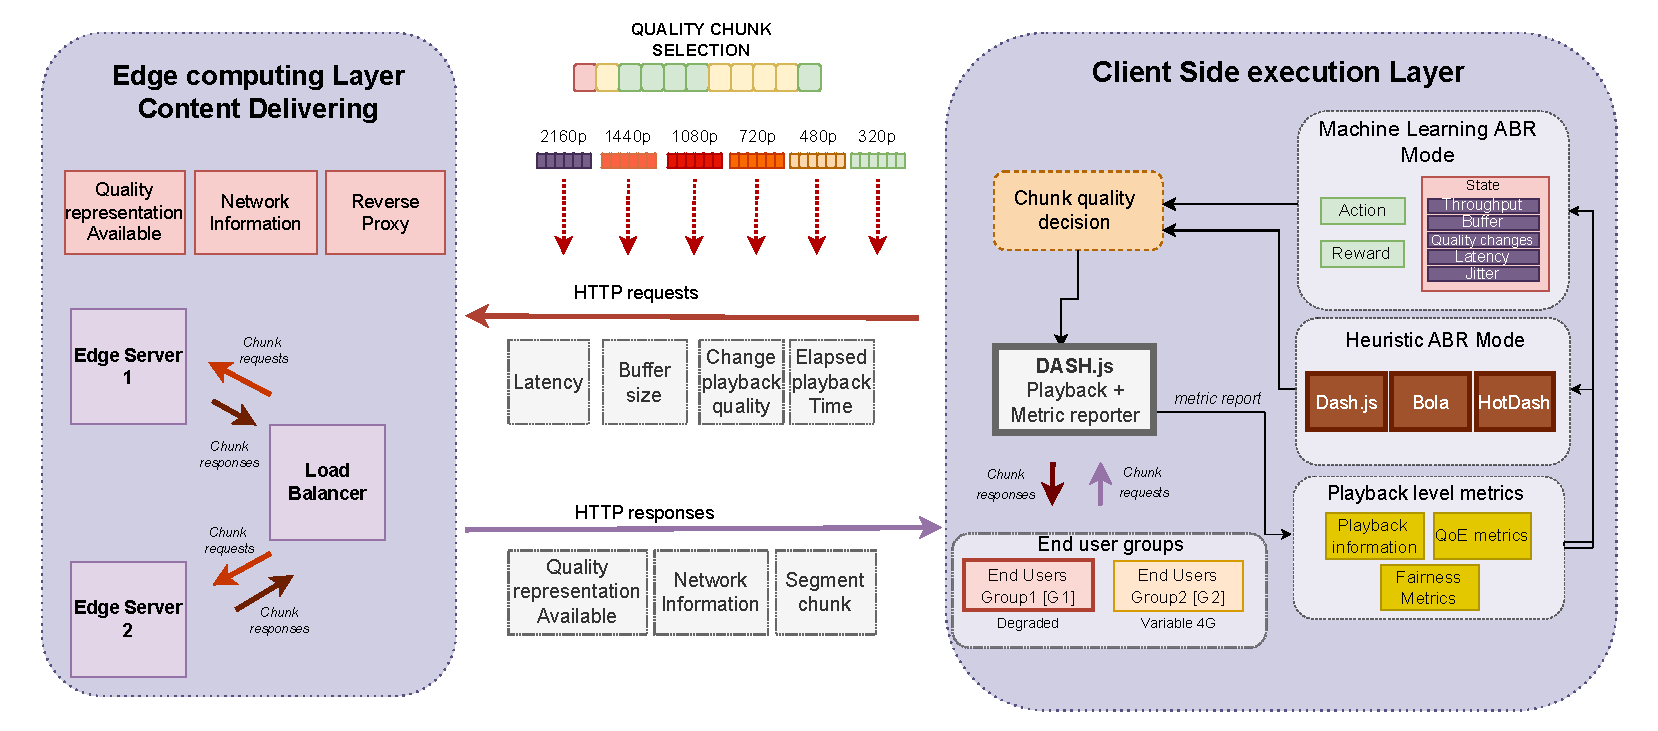
\includegraphics[scale=0.20]{experiment-01-general-architecture.pdf}
        \caption{Arquitetura Geral do Experimento.}
    \end{figure}
    
    \subsubsection*{Resultados de Aprendizagem}
    \begin{itemize}
        \item Entender a virtualização do sistema e navegação básica.
    \end{itemize}
\end{boxTutorial}
    
    
\newpage  
\begin{boxTutorial}{Tutorial 2: Uso do Terminal no Raspberry Pi OS via UTM}
    \label{sec: Etapa 2: Uso do Terminal no Raspberry Pi OS via UTM}
        Introdução ao terminal Linux: comandos básicos, instalação de pacotes e execução de scripts Python.
        
        \subsubsection*{Objetivos}
        \begin{itemize}
            \item Abrir e utilizar o terminal do Raspberry Pi OS.
            \item Instalar pacotes com \texttt{apt} e executar scripts Python.
        \end{itemize}
        
    \begin{minted}{bash}
sudo apt-get update && sudo apt-get upgrade
sudo apt-get install python3 python3-pip -y
python3 ola.py
    \end{minted}
        
        \subsubsection*{Resultados de Aprendizagem}
        \begin{itemize}
            \item Autonomia no gerenciamento de arquivos e execução de software via CLI.
        \end{itemize}
\end{boxTutorial}
    

\newpage

\begin{boxTutorial}{Tutorial 3: Design do Jogo e Feedback Musical}
\label{sec: Etapa 3: Design do Jogo e Feedback Musical}

    \begin{minted}{python}
pygame.mixer.init()
screen = pygame.display.set_mode((400, 300))
pygame.display.set_caption("Teste de Sons")

som_acerto = pygame.mixer.Sound("acerto.wav")
som_erro = pygame.mixer.Sound("erro.wav")

rodando = True
while rodando:
    for evento in pygame.event.get():
        if evento.type == pygame.QUIT:
            rodando = False
        if evento.type == pygame.KEYDOWN:
            if evento.key == pygame.K_a:
                som_acerto.play()
            elif evento.key == pygame.K_e:
                som_erro.play()

pygame.quit()
    \end{minted}
\end{boxTutorial}

\subsubsection*{Primeiros Exercícios Práticos}
\begin{itemize}
    \item Criar um script que toque diferentes sons com base em teclas pressionadas.
    \item Trocar os sons por opções escolhidas no tutorial anterior.
    \item Criar variações para testar sons diferentes em sequência.
\end{itemize}

\subsubsection*{Resultados de Aprendizagem Esperados}
\begin{itemize}
    \item Compreender como integrar eventos do teclado com reprodução de sons em Python.
    \item Criar um programa básico, mas funcional, com estrutura de loops, condicionais e eventos.
    \item Preparar terreno para expansão do código em forma de jogo ou aplicação educacional.
\end{itemize}

\newpage
\begin{boxTutorial}{Tutorial 5: Telas e Gráficos com Pygame}
\label{sec:tutorial5}

    Nesta etapa inicia-se a implementação em Python utilizando a biblioteca \texttt{pygame}. O objetivo é criar a janela principal, o laço de execução e um estímulo visual (estrela piscando).
    
    \subsubsection*{Guia de Aprendizagem}
    \begin{enumerate}
        \item Criar a pasta do projeto e o ambiente virtual:
    \begin{minted}{bash}
mkdir -p ~/projetos/musicalizando && cd ~/projetos/musicalizando
python3 -m venv .venv
source .venv/bin/activate
pip install pygame
    \end{minted}
    
        \item Código base para a estrela piscando:
    \begin{minted}{python}
import pygame, sys
WIDTH, HEIGHT = 800, 480
FPS = 60

def main():
    pygame.init()
    screen = pygame.display.set_mode((WIDTH, HEIGHT))
    clock = pygame.time.Clock()
    blink_timer = 0.0
    star_visible = True

    while True:
        dt = clock.tick(FPS) / 1000.0
        for event in pygame.event.get():
            if event.type == pygame.QUIT: pygame.quit(); sys.exit()

        blink_timer += dt
        if blink_timer >= 0.8:
            star_visible = not star_visible; blink_timer = 0.0

        screen.fill((20, 30, 80))
        if star_visible:
            pygame.draw.circle(screen, (255, 215, 0), (WIDTH//2, HEIGHT//2), 30)
        pygame.display.flip()

if __name__ == "__main__": main()
    \end{minted}
    \end{enumerate}
    
    \subsubsection*{Exercícios Práticos}
    \begin{itemize}
        \item Alterar o tamanho e a velocidade do piscar da estrela.
        \item Posicionar duas estrelas em ritmos diferentes.
    \end{itemize}
\end{boxTutorial}

\newpage
\begin{boxTutorial}{Tutorial 6: Score e Feedback de Estímulo-Resposta}
\label{sec: Etapa 6: Interação}

    Mapeamento de entrada do usuário (teclado/clique) e associação com feedback positivo/negativo.
    
    \subsubsection*{Guia de Aprendizagem}
    \begin{enumerate}
        \item Testar o áudio no Raspberry Pi:
        \begin{minted}{python}
import pygame
pygame.mixer.init()
s = pygame.mixer.Sound("acerto.wav")
s.play()
        \end{minted}
    
        \item Mapear tecla 'A' para acerto:
        \begin{minted}{python}
if event.type == pygame.KEYDOWN and event.key == pygame.K_a:
    if star_visible:
        pontos += 1; acerto_snd.play()
    else:
        pontos = max(0, pontos-1); erro_snd.play()
        \end{minted}
    \end{enumerate}
    
    \subsubsection*{Exercícios Práticos}
    \begin{itemize}
        \item Adicionar feedback visual (ex: borda verde para acerto, vermelha para erro).
        \item Exibir a pontuação atualizada na tela usando \texttt{pygame.font}.
    \end{itemize}
\end{boxTutorial}

\newpage
\begin{boxTutorial}{Tutorial 7: Fases e Progressão de Sequências}
\label{sec: Etapa 7: Fases e Progressão de Sequências}

    Nesta etapa organizamos a lógica de fases, adicionamos sequências (listas de estímulos) e tempo-limite de resposta. Ao completar a sequência, a fase é concluída e pode-se avançar.
    
    \subsubsection*{Objetivos}
    \begin{itemize}
        \item Definir fases com parâmetros (nº de estímulos, tempo de resposta, velocidade).
        \item Implementar sequência de alvos e avaliação de acerto dentro do tempo.
        \item Exibir barra de progresso ou contador de acertos da fase.
    \end{itemize}
    
    \subsubsection*{Requisitos}
    \begin{itemize}
        \item Concluir as Etapas 5 e 6.
    \end{itemize}
    
    \subsubsection*{Guia de Aprendizagem}
    \begin{enumerate}
        \item Criar um arquivo de configuração simples (\texttt{levels.py}) com as fases:
    \begin{minted}{python}
# levels.py
LEVELS = [
    {"name": "Fase 1", "seq_len": 4, "blink_period": 0.9, "timeout": 2.8},
    {"name": "Fase 2", "seq_len": 6, "blink_period": 0.7, "timeout": 2.0},
    {"name": "Fase 3", "seq_len": 8, "blink_period": 0.55, "timeout": 1.5},
]
    \end{minted}
    
        \item Atualizar \texttt{main.py} para controlar sequência, tempo e progresso:
    \begin{minted}{python}
import pygame, sys, random, time
from levels import LEVELS

WIDTH, HEIGHT = 800, 480
FPS = 60
SKY = (20, 30, 80)
WHITE = (245, 245, 245)
GOLD = (255, 215, 0)
GREEN= (60, 180, 75)
RED  = (200, 60, 60)

def desenhar_estrela(surface, x, y, size, color):
    # Desenha um polígono estelar de 5 pontas
    pts = [(x, y - size), (x + size*0.3, y - size*0.3), (x + size, y - size*0.3),
           (x + size*0.45, y + size*0.1), (x + size*0.6, y + size),
           (x, y + size*0.45), (x - size*0.6, y + size),
           (x - size*0.45, y + size*0.1), (x - size, y - size*0.3),
           (x - size*0.3, y - size*0.3)]
    pygame.draw.polygon(surface, color, pts)

def main():
    pygame.init(); pygame.mixer.init()
    screen = pygame.display.set_mode((WIDTH, HEIGHT))
    pygame.display.set_caption("Musicalizando no Céu - Fases")
    clock = pygame.time.Clock()
    font = pygame.font.SysFont(None, 26)

    # Carregar sons (Certifique-se de que os arquivos existem em assets/sounds/)
    # acerto_snd = pygame.mixer.Sound("assets/sounds/acerto.wav")
    # erro_snd   = pygame.mixer.Sound("assets/sounds/erro.wav")

    level_idx = 0; pontos = 0

    while level_idx < len(LEVELS):
        level = LEVELS[level_idx]
        seq_len = level["seq_len"]; blink_per = level["blink_period"]; timeout_s = level["timeout"]
        sequence = [random.choice([0,1]) for _ in range(seq_len)]
        seq_pos = 0; star_visible = False; blink_timer = 0.0; stim_timer = 0.0
        feedback_color = None; feedback_timer = 0.0; responded = False

        running_phase = True
        while running_phase:
            dt = clock.tick(FPS)/1000.0
            for event in pygame.event.get():
                if event.type == pygame.QUIT: pygame.quit(); sys.exit()
                if event.type == pygame.KEYDOWN and event.key == pygame.K_a:
                    if not responded:
                        responded = True
                        if star_visible:
                            pontos += 1; feedback_color = GREEN
                        else:
                            pontos = max(0, pontos-1); feedback_color = RED
                        feedback_timer = 0.3

            # Lógica de piscar e sequência
            blink_timer += dt
            if blink_timer >= blink_per:
                blink_timer = 0.0
                if seq_pos < seq_len:
                    star_visible = bool(sequence[seq_pos]); seq_pos += 1
                    responded = False; stim_timer = 0.0
            
            # Fim da fase
            if seq_pos >= seq_len and responded: running_phase = False

            # Renderização
            screen.fill(SKY)
            color = GOLD if star_visible else WHITE
            desenhar_estrela(screen, WIDTH//2, HEIGHT//2, 30, color)
            
            # HUD e Progresso
            prog_w = int((seq_pos/seq_len) * (WIDTH-40))
            pygame.draw.rect(screen, WHITE, (20, 20, WIDTH-40, 10), 1)
            pygame.draw.rect(screen, GREEN, (20, 20, prog_w, 10))
            header = font.render(f"{level['name']} | Pontos: {pontos}", True, WHITE)
            screen.blit(header, (20, 40))
            
            if feedback_color:
                pygame.draw.rect(screen, feedback_color, (0, 0, WIDTH, 5))
                feedback_timer -= dt
                if feedback_timer <= 0: feedback_color = None
            
            pygame.display.flip()
        level_idx += 1
    pygame.quit()

if __name__ == "__main__": main()
    \end{minted}
    \end{enumerate}

    \subsubsection*{Exercícios Práticos}
    \begin{itemize}
        \item Trocar a regra da sequência para notas (ex.: 3 sons diferentes).
        \item Ajustar \texttt{seq\_len} e \texttt{timeout} no arquivo \texttt{levels.py}.
        \item Exibir uma tela de ``Fase Concluída'' com o score final.
    \end{itemize}

    \subsubsection*{Resultados de Aprendizagem Esperados}
    \begin{itemize}
        \item Controle de fluxo por fases e temporização por estímulo.
        \item Implementação de progressão e finalização de fase.
    \end{itemize}
\end{boxTutorial}

\newpage
\begin{boxTutorial}{Tutorial 8: Tela Inicial e Registro do Jogador}
\label{sec: Tutorial 8: Tela Inicial}

    Esta etapa implementa a tela inicial minimalista: campos para \textbf{Nome} e \textbf{Escola}.
    
    \subsubsection*{Objetivos}
    \begin{itemize}
    \item Exibir tela inicial com campos de texto e botão "Começar".
    \item Validar entradas antes de avançar.
    \end{itemize}
    
    \begin{minted}{python}
while mode == "menu":
    # ... lógica de entrada de texto ...
    if button_rect.collidepoint(event.pos):
        if player_name.strip() and player_school.strip():
            mode = "phase1"
    \end{minted}
    
    \subsubsection*{Resultados de Aprendizagem Esperados}
    \begin{itemize}
    \item Entender a interação básica entre UI, eventos e estado do jogo.
    \item Ter um fluxo de entrada do jogador funcional que inicia a Fase 1.
    \item Preparar o terreno para implementar a lógica da Fase 1 no próximo tutorial.
\end{boxTutorial}


\newpage
\begin{boxTutorial}{Tutorial 9: Fase 1 com Score e Feedback}
\label{sec: Tutorial 9: Fase 1}

    Implementação da mecânica básica: quatro alvos (setas), um alvo destacado por rodada e atualização do placar.
    
    \subsubsection*{Objetivos}
    \begin{itemize}
    \item Implementar a lógica de estímulo-resposta.
    \item Exibir HUD com Nome, Escola e Pontuação.
    \end{itemize}
    
    \begin{minted}{python}
if event.key in STAR_KEYS:
    if event.key == target_key:
        score += 1
        feedback = "ACERTOU"
    \end{minted}
    
    \subsubsection*{Resultados de Aprendizagem}
    \begin{itemize}
    \item Interação dinâmica e feedback imediato em tempo real.
    \end{itemize}
\end{boxTutorial}

\newpage
\begin{boxTutorial}{Tutorial 10: Interação com Botões (GPIO)}
\label{sec:Tutorial10_Botoes}

    Integração de botões físicos via \textbf{GPIO} e alternativas de simulação via software para desenvolvimento em ambientes sem hardware.
    
    \subsubsection*{Dicas Técnicas}
    \begin{itemize}
        \item Sempre use apenas 3.3V nos GPIOs (não use 5V).
        \item Botões simples devem ser conectados entre o pino GPIO e GND, com pull-up interno habilitado.
    \end{itemize}
    
    \subsubsection*{Guia de Aprendizagem}
    \begin{enumerate}
        \item Exemplo de botão físico com \texttt{gpiozero}:
        \begin{minted}{python}
from gpiozero import Button
def on_hw_button():
    print("Botão físico pressionado!")

btn = Button(17, pull_up=True, bounce_time=0.05)
btn.when_pressed = on_hw_button
        \end{minted}

        \item Exemplo de Mock GPIO (para testes locais em PC):
        \begin{minted}{python}
from gpiozero import Device, Button
from gpiozero.pins.mock import MockFactory
Device.pin_factory = MockFactory()
btn = Button(17, pull_up=True)

# Simular pressão via código
pin = Device.pin_factory.pin(17)
pin.drive_low(); pin.drive_high()
        \end{minted}
    \end{enumerate}
    
    \subsubsection*{Exercícios Práticos}
    \begin{itemize}
        \item Adicionar um segundo botão para ``Pausar'' o jogo.
        \item Registrar timestamps de pressões em CSV (tempo de reação).
    \end{itemize}
\end{boxTutorial}

\begin{boxTutorial}{Tutorial 11: Layout Dinâmico e Responsivo}
\label{sec:Tutorial11_LayoutDinamico}

    Nesta etapa aprendemos a posicionar elementos de forma relativa ao tamanho da tela, permitindo que o jogo rode em diferentes resoluções.
    
    \subsubsection*{Guia de Aprendizagem}
    \begin{enumerate}
        \item Criar uma função auxiliar para calcular posições relativas:
        \begin{minted}{python}
def pos_rel(x_frac, y_frac, width, height):
    """ Retorna posição relativa dado percentual da tela """
    return int(width * x_frac), int(height * y_frac)
        \end{minted}
    
        \item Criar botões com base em porcentagens:
        \begin{minted}{python}
WIDTH, HEIGHT = 900, 600
start_btn_rect = pygame.Rect(0, 0, WIDTH//4, HEIGHT//12)
start_btn_rect.center = pos_rel(0.5, 0.7, WIDTH, HEIGHT)
        \end{minted}
    \end{enumerate}
    
    \subsubsection*{Exercícios Práticos}
    \begin{itemize}
        \item Criar uma função \texttt{resize\_ui()} para reposicionamento dinâmico.
        \item Testar o jogo em diferentes resoluções (fullscreen, 1280x720).
    \end{itemize}
\end{boxTutorial}

\begin{boxTutorial}{Tutorial 12: Trilha Sonora e Ambiência}
\label{sec: Etapa 12: Criação e Edição de Trilha Sonora no Jogo}

Nesta etapa, Luisa aprenderá a incorporar sons ao jogo, criando músicas de fundo e efeitos específicos para eventos de vitória e derrota.

\subsubsection*{Checklist de Atividades}
\begin{itemize}
    \item [ ] Escolher trilha, som de vitória e som de derrota (BeepBox/Mixkit).
    \item [ ] Salvar arquivos em \texttt{.mp3} ou \texttt{.wav} na pasta \texttt{./sounds/}.
    \item [ ] Inserir código Python para reprodução sonora.
\end{itemize}

\subsubsection*{Sites Recomendados}
\begin{itemize}
    \item \href{https://freesound.org}{Freesound.org} – Efeitos e sons gratuitos [\textit{prontos para baixar}].
    \item \href{https://beepbox.co}{BeepBox.co} – Cria melodias curtas em estilo 8-bit [\textit{para criação própria}].
    \item \href{https://soundtrap.com}{Soundtrap.com} – Editor online para trilhas elaboradas.
\end{itemize}
    
    \begin{minted}{python}
pygame.mixer.music.load("sounds/trilha_fase.mp3")
pygame.mixer.music.play(-1) # Loop infinito
    \end{minted}

    \begin{figure}[H]
        \centering
        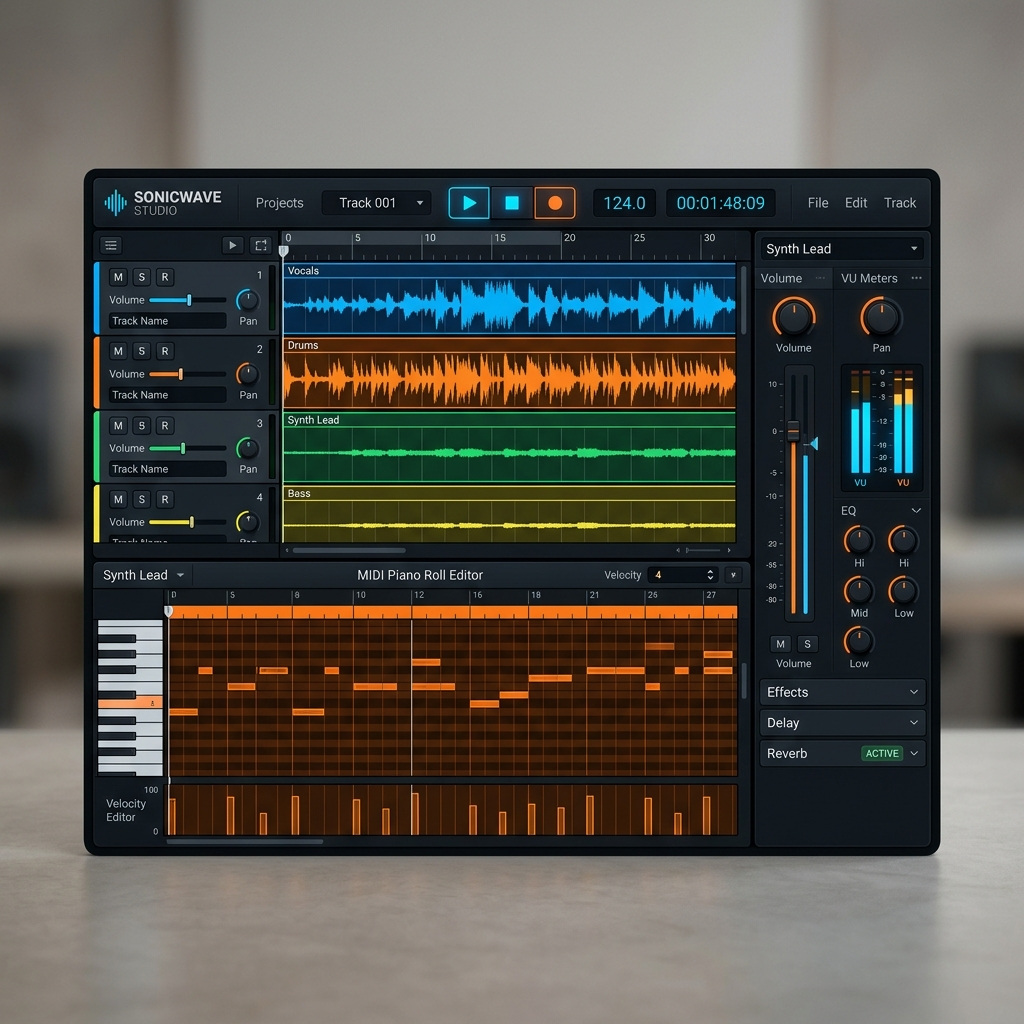
\includegraphics[width=0.85\linewidth]{soundtrap_ui.png}
        \caption{Interface do Soundtrap: ferramenta para criação de trilhas sonoras complexas.}
        \label{fig:soundtrap-ui}
    \end{figure}
    
    \begin{boxAvisos}{Feedback e Gamificação}
    A utilização estratégica de áudio e visual (fanfarras, ícones de vitória) reforça o engajamento e o aprendizado atencional.
\end{boxAvisos}

\subsubsection*{Resultados de Aprendizagem}
\begin{itemize}
    \item Uso estratégico de áudio para reforçar o engajamento e feedback.
\end{itemize}

\subsubsection*{Conclusão}
Com esta etapa, o jogo passa a ter um componente sonoro dinâmico que reforça o envolvimento da jogadora.
\end{boxTutorial}


\newpage

\newpage
\begin{boxTutorial}{Tutorial 13: Introdução ao BeepBox e Tema Mario}
\label{sec:tutorial13}

    Apresentação do \textbf{BeepBox} para criação de trilhas 8-bit e recriação do tema do \textit{Super Mario Bros.} em versão simplificada.
    
    \subsubsection*{Guia Musical (Mario Theme)}
    \begin{verbatim}
E E - E - C E - G - - - G
C - G - E - A B A A - -
    \end{verbatim}
    
    \subsubsection*{Resultados de Aprendizagem}
    \begin{itemize}
        \item Compreensão de melodia, ritmo e exportação de áudio para jogos.
    \end{itemize}

    \begin{figure}[H]
        \centering
        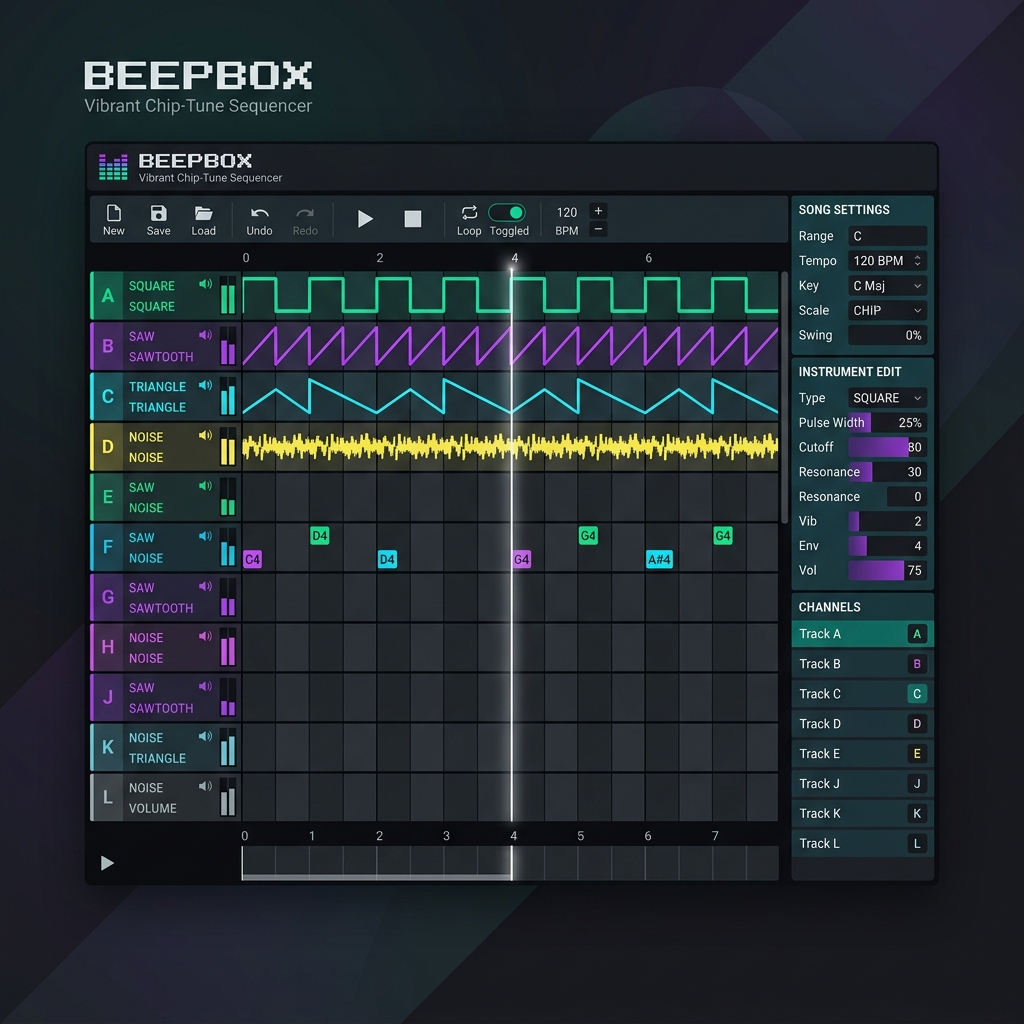
\includegraphics[width=0.85\linewidth]{beepbox_ui.png}
        \caption{Interface do BeepBox para criação de trilhas 8-bit.}
        \label{fig:beepbox-ui}
    \end{figure}
\end{boxTutorial}

\begin{boxTutorial}{Tutorial: Fluxo de Trabalho Git}
\label{sec:fluxo-trabalho-git}

    Guia para versionamento colaborativo utilizando Git e GitHub.
    
    \subsubsection*{Objetivos}
    \begin{itemize}
        \item Sincronizar o código entre diferentes máquinas.
        \item Manter o histórico de versões seguro.
    \end{itemize}
    
    \begin{minted}{bash}
git add .
git commit -m "Mensagem clara"
git push origin main

# 3. Ver o que mudou
git status

# 4. Adicionar as alterações
git add .

# 5. Criar o commit
git commit -m "Mensagem clara"

# 6. Enviar para o GitHub
git push origin main
    \end{minted}

    \begin{figure}[H]
        \centering
        \begin{tikzpicture}[
            node distance=2.5cm,
            every node/.style={font=\scriptsize, align=center},
            box/.style={rectangle, rounded corners, draw=azulIFSC!70, thick, fill=azulIFSC!5, minimum width=2cm, minimum height=1cm},
            arrow/.style={-{Stealth[length=2mm]}, thick, draw=azulIFSC!70}
        ]
            \node[box] (edit) {Editar};
            \node[box, right of=edit] (add) {Add};
            \node[box, right of=add] (commit) {Commit};
            \node[box, right of=commit] (push) {Push};
            \node[box, below of=commit, yshift=-1cm] (pull) {Pull};
            \draw[arrow] (edit) -- (add);
            \draw[arrow] (add) -- (commit);
            \draw[arrow] (commit) -- (push);
            \draw[arrow] (push) |- (pull);
            \draw[arrow] (pull) -| (edit);
        \end{tikzpicture}
        \caption{Ciclo de desenvolvimento com Git.}
    \end{figure}

    \subsubsection*{Conclusão}
    Seguindo este fluxo, cada colaborador pode trabalhar de forma independente e sincronizada.
\end{boxTutorial}



\newpage
\begin{boxTutorial}{Tutorial 14: SSH e Cabo RJ45}
\label{sec: Tutorial 14: Acesso Remoto SSH}

    Estabelecimento de conexão direta entre Raspberry Pi e Computador para configuração inicial.
    
    \subsubsection*{Objetivos}
    \begin{itemize}
        \item Acessar o terminal via SSH.
        \item Ativar o serviço sem monitor/teclado.
    \end{itemize}
    
    \begin{minted}{bash}
ssh pi@raspberrypi.local
    \end{minted}
    
    \subsubsection*{Dica de Ouro}
    \textit{Crie um arquivo vazio chamado \texttt{ssh} na partição boot do SD para ativar o acesso automático.}
\end{boxTutorial}



\newpage
\begin{boxTutorial}{Tutorial 15: Acesso Gráfico via VNC}
\label{sec: Tutorial 15: VNC}

    Acesso ao desktop do Raspberry Pi para facilitar o desenvolvimento visual.
    
    \subsubsection*{Objetivos}
    \begin{itemize}
        \item Ativar VNC Server via \texttt{raspi-config}.
        \item Conectar usando VNC Viewer.
    \end{itemize}
    
    \begin{minted}{bash}
sudo raspi-config # Interface Options -> VNC -> Enable
    \end{minted}
\end{boxTutorial}



\printbibliography[title={Referências}]

\newpage

\begin{boxAvisos}{Checklist de Revisão Estrutural}
    \label{sec:checklist-revisao}
    
    Esta seção contém os modelos de reescrita e ajustes formais necessários para a padronização acadêmica do documento.

\subsection*{1. Abstract}

\begin{itemize}
    \item[$\boxtimes$] Substituir expressões fortes como ``comprovada a eficácia'' por termos como ``avaliada a viabilidade''.
    
    \textbf{Modelo de Reescrita:}
    
    \textit{``para que possa ser avaliada a viabilidade e o impacto preliminar da ferramenta proposta.''}

    \item[$\boxtimes$] Reformular ``potencial pedagógico'' para linguagem não conclusiva.
    
    \textbf{Modelo de Reescrita:}
    
    \textit{``Espera-se que a ferramenta apresente indícios de viabilidade pedagógica em contexto educacional.''}

    \item[$\boxtimes$] Inserir frase explícita indicando que a proposta não substitui tratamento clínico ou farmacológico.
    
    \textbf{Modelo de Inserção:}
    
    \textit{``Ressalta-se que a proposta não substitui intervenções clínicas ou farmacológicas, atuando como ferramenta complementar de apoio educacional.''}

    \item[$\boxtimes$] Tornar mais claro o delineamento metodológico previsto.
    
    \textbf{Modelo de Inserção:}
    
    \textit{``O estudo prevê delineamento quase-experimental com comparação entre condições com e sem estímulo musical estruturado.''}
\end{itemize}

% ------------------------------------------------------

\subsection*{2. Introdução}

\begin{itemize}
    \item[$\boxtimes$] Reescrever o parágrafo que inicia com ``Diferentemente da abordagem medicinal tradicional...'' evitando comparação direta com medicina tradicional.
    
    \textbf{Modelo de Reescrita:}
    
    \textit{``Além das intervenções farmacológicas amplamente utilizadas, pesquisas recentes indicam que abordagens complementares baseadas em estímulos cognitivos e musicais podem contribuir para o desenvolvimento da atenção em crianças com TDAH.''}

    \item[$\boxtimes$] Inserir hipótese formal da pesquisa.
    
    \textbf{Modelo de Inserção:}
    
    \textit{``A hipótese central deste estudo é que crianças expostas a estímulos musicais estruturados durante atividades interativas apresentarão melhor desempenho em tarefas de atenção sustentada quando comparadas à condição sem estímulo musical estruturado.''}

    \item[$\boxtimes$] Definir variáveis independentes (tipo de estímulo musical).
    
    \textbf{Modelo de Inserção:}
    
    \textit{``A variável independente corresponde ao tipo de estímulo musical aplicado durante a atividade.''}

    \item[$\boxtimes$] Definir variáveis dependentes (tempo de resposta, número de acertos, evolução por fase).
    
    \textbf{Modelo de Inserção:}
    
    \textit{``As variáveis dependentes incluem tempo de resposta, taxa de acertos e evolução do desempenho ao longo das fases do jogo.''}

    \item[$\boxtimes$] Reforçar explicitamente que a proposta é complementar ao tratamento clínico.
    
    \textbf{Modelo de Inserção:}
    
    \textit{``A proposta apresentada possui caráter complementar, não substituindo intervenções clínicas ou terapêuticas previamente estabelecidas.''}
\end{itemize}

% ------------------------------------------------------

\subsection*{3. Fundamentação Teórica}

\begin{itemize}
    \item[$\boxtimes$] Substituir termos como ``portador do transtorno'' por ``criança com TDAH''.
    
    \textbf{Modelo de Substituição:}
    
    \textit{Trocar todas as ocorrências de ``portador do transtorno'' por ``criança com TDAH''.}

    \item[$\boxtimes$] Inserir referências recentes (2022--2025).
    
    \textbf{Modelo de Inserção:}
    
    \textit{Inserir estudos recentes que abordem música e atenção, intervenções não farmacológicas no TDAH e jogos digitais cognitivos.}

    \item[$\boxtimes$] Remover a Tabela comparativa Arduino vs Raspberry Pi.
    
    \item[$\boxtimes$] Substituir a tabela por um parágrafo técnico objetivo justificando a escolha do Raspberry Pi.
    
    \textbf{Modelo de Inserção:}
    
    \textit{``A escolha do Raspberry Pi deve-se à sua maior capacidade de processamento, compatibilidade com bibliotecas multimídia como Pygame e possibilidade de registro automatizado de métricas atencionais em tempo real.''}
\end{itemize}

% ------------------------------------------------------

\subsection*{4. Trabalhos Relacionados}

\begin{itemize}
    \item[$\Box$] Tornar a análise dos GAPS mais crítica e aprofundada.
    
    \item[$\Box$] Inserir parágrafo final explicitando claramente a contribuição original do trabalho.
    
    \textbf{Modelo de Inserção:}
    
    \textit{``Diferentemente dos trabalhos analisados, esta proposta integra estímulos musicais estruturados, coleta automatizada de métricas atencionais e aplicação em ambiente educacional, configurando uma abordagem interdisciplinar entre tecnologia acessível e intervenção cognitiva.''}

    \item[$\Box$] Evitar linguagem superficial ou apenas descritiva.
\end{itemize}

% ------------------------------------------------------

\subsection*{5. Metodologia}

\begin{itemize}
    \item[$\boxtimes$] Especificar o tipo de estudo.
    
    \textbf{Modelo de Inserção:}
    
    \textit{``O estudo caracteriza-se como quase-experimental, com delineamento comparativo entre duas condições experimentais.''}

    \item[$\boxtimes$] Inserir descrição formal do delineamento experimental.
    
    \item[$\boxtimes$] Considerar inclusão de grupo controle.
    
    \textbf{Modelo de Inserção:}
    
    \textit{``Os participantes poderão ser divididos em Grupo Experimental (com estímulo musical estruturado) e Grupo Controle (sem estímulo musical adicional), permitindo comparação entre condições.''}

    \item[$\Box$] Especificar testes estatísticos previstos.
    
    \textbf{Modelo de Inserção:}
    
    \textit{``Os dados serão analisados por meio de teste t para comparação entre médias e ANOVA para análise entre fases, adotando-se nível de significância de $p < 0{,}05$.''}

    \item[$\boxtimes$] Substituir expressões especulativas como ``será possível observar''.
    
    \textbf{Modelo de Substituição:}
    
    \textit{Trocar por: ``serão analisadas variações nos indicadores de desempenho atencional''.}
\end{itemize}

% ------------------------------------------------------

\subsection*{6. Design do Jogo}

\begin{itemize}
    \item[$\Box$] Especificar parâmetros técnicos dos estímulos sonoros.
    
    \textbf{Modelo de Inserção:}
    
    \textit{``Os estímulos sonoros serão configurados com frequência entre 400Hz e 800Hz, duração média de 300ms, ritmo entre 60 e 90 BPM e intervalo aproximado de 2 segundos entre estímulos.''}
\end{itemize}

% ------------------------------------------------------

\subsection*{7. Ferramentas Utilizadas}

\begin{itemize}
    \item[$\Box$] Especificar modelo do Raspberry Pi.
    
    \textbf{Modelo de Inserção:}
    
    \textit{``O sistema foi desenvolvido utilizando Raspberry Pi 4 Model B.''}

    \item[$\boxtimes$] Informar versão do Python e Pygame.
    
    \textbf{Modelo de Inserção:}
    
    \textit{``Foram utilizadas as versões Python 3.11 e Pygame 2.x.''}

    \item[$\boxtimes$] Inserir link para repositório.
    
    \textbf{Modelo de Inserção:}
    
    \textit{``O código-fonte será disponibilizado em repositório público para fins de reprodutibilidade científica.''}
\end{itemize}

% ------------------------------------------------------

\subsection*{8. Aspectos Éticos}

\begin{itemize}
    \item[$\Box$] Criar subseção específica sobre Aspectos Éticos.
    
    \textbf{Modelo de Texto:}
    
    \textit{``A participação ocorrerá mediante consentimento livre e esclarecido dos responsáveis legais e assentimento das crianças. Os dados serão anonimizados por meio de identificação alfanumérica, não sendo armazenadas informações pessoais sensíveis. O armazenamento seguirá as diretrizes da Lei Geral de Proteção de Dados (LGPD). Caso aplicável, o projeto será submetido a Comitê de Ética em Pesquisa.''}
\end{itemize}

% ------------------------------------------------------

\subsection*{9. Resultados}

\begin{itemize}
    \item[$\boxtimes$] Avaliar renomear seção para ``Plano de Avaliação Experimental''.
    
    \item[$\boxtimes$] Substituir termos como ``comprovam''.
    
    \textbf{Modelo de Substituição:}
    
    \textit{Trocar por: ``indicam viabilidade técnica preliminar do sistema''.}

    \item[$\boxtimes$] Reduzir linguagem afirmativa sobre eficácia.
\end{itemize}

% ------------------------------------------------------

\subsection*{10. Considerações Finais}

\begin{itemize}
    \item[$\boxtimes$] Reformular linguagem conclusiva.
    
    \textbf{Modelo de Reescrita:}
    
    \textit{``Os resultados obtidos até o momento indicam viabilidade técnica do sistema, sendo necessária validação experimental com amostra ampliada para avaliação do impacto atencional.''}

    \item[$\boxtimes$] Destacar necessidade de validação futura.
\end{itemize}

% ------------------------------------------------------

\subsection*{11. Ajustes Formais}

\begin{itemize}
    \item[$\boxtimes$] Corrigir ``Figure'' para ``Figura''.
    \item[$\boxtimes$] Corrigir ``Table'' para ``Tabela''.
    \item[$\Box$] Atualizar campos CCSXML.
    \item[$\Box$] Revisão gramatical completa.
\end{itemize}


\end{boxAvisos}

\end{document}